
%(BEGIN_QUESTION)
% Copyright 2012, Tony R. Kuphaldt, released under the Creative Commons Attribution License (v 1.0)
% This means you may do almost anything with this work of mine, so long as you give me proper credit

Dette koblingsdiagrammet viser en enkel trykkreguleringssløyfe der en 4-20 mA loop-powered transmitter sender signal til Honeywell-regulator, som igjen sender 4-20 mA til reguleringsventil:

$$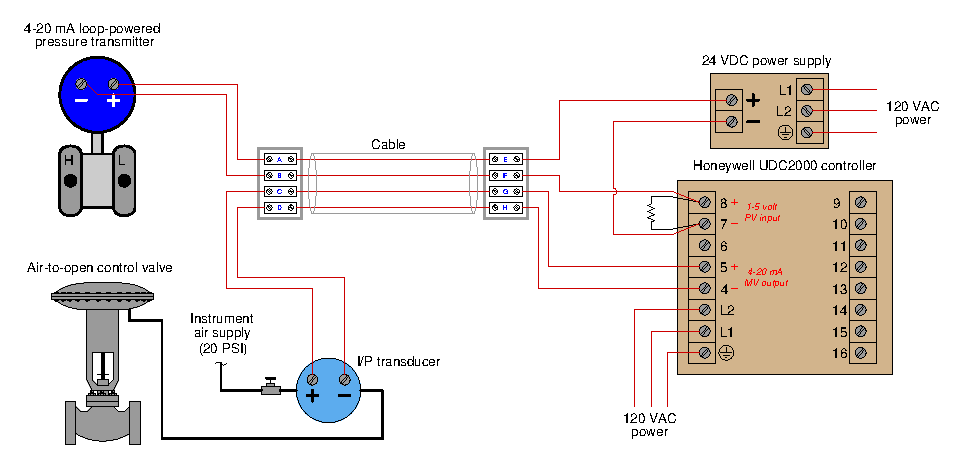
\includegraphics[width=15.5cm]{i00974x01.eps}$$

\begin{itemize}
\item{} Skisser strømretning med konvensjonell strømretning.
\vskip 10pt
\item{} Angi hvilke enheter som er {\it kilder} og hvilke som er {\it laster}.
\vskip 10pt
\item{} Hvis regulatoren viser underrange ($-25$\%), hvilke elektriske feil kan mistenkes? Finnes ikke-elektriske årsaker?
\vskip 10pt
\item{} Hvis ventilen forblir helt stengt uansett regulatorutgang (også i manuell), hvilke feil kan mistenkes?
\vskip 10pt
\item{} Anta kortslutning mellom transmitterledere i kabelen. Forklar effekt på systemet og hvordan du kan bevise at feilen sitter i kabelen (ikke transmitter) med kun voltmeter.
\end{itemize}

\vskip 20pt \vbox{\hrule \hbox{\strut \vrule{} {\bf Forslag til sokratisk diskusjon} \vrule} \hrule}

\begin{itemize}
\item{} Gå gjennom problemløsningstipsene i spørsmål 0 og bruk dem her.
\end{itemize}


\underbar{file i00974}
%(END_QUESTION)





%(BEGIN_ANSWER)

$$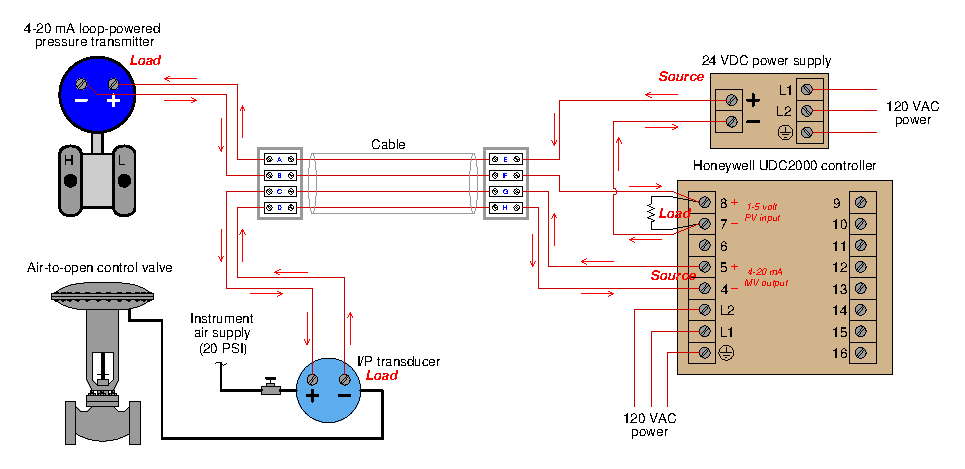
\includegraphics[width=15.5cm]{i00974x02.eps}$$

Selv om loop-powered transmitter regulerer strømmen, er den en {\it last} og ikke en {\it kilde}. 24 VDC-forsyningen er energikilden i kretsen.
 
\vskip 10pt

Full nedskala ($-25$\%) tyder på {\it åpen} feil i transmitterkretsen (tilsvarer 0 mA).

\vskip 10pt

Uresponsiv reguleringsventil tyder på manglende luft til membran. Dette kan skyldes elektrisk feil i utgangskretsen, svikt i luftforsyning eller mekanisk feil i I/P.

\vskip 10pt

Kortslutning i transmitterkabling gir fullskala strøm ($>$20 mA). Med kun voltmeter må kretsen brytes og spenning måles oppstrøms for å lokalisere om kortslutning ligger nedstrøms.

%(END_ANSWER)





%(BEGIN_NOTES)

%INDEX% Pictorial circuit review (4-20 mA loop)
%INDEX% Troubleshooting review: electric circuits

%(END_NOTES)

